\documentclass[11pt]{article}
\usepackage{a4wide}
\usepackage{float}
\usepackage{graphicx}
\usepackage{hyperref}
\usepackage[margin=0.95in,footskip=0.25in]{geometry}
\graphicspath{{./images/}}
\usepackage[dutch]{babel}
\usepackage{graphicx}
\usepackage{subfig}
\usepackage{lipsum}
\usepackage{booktabs}
\usepackage[utf8]{inputenc}
\usepackage{float}
\usepackage{tabularx}
\begin{document}

\begin{titlepage}
\title{Reinforcement learning gebaseerde agent voor presidenten}
\author{Freya Van Speybroek \& Thor Dossche}
\date{Academiejaar 2020 \- 2021}
\maketitle
\thispagestyle{empty}
\end{titlepage}


\section{Inleiding}
In dit project zullen we bestuderen hoe reinforcement learning kan toegepast worden op een kaartspel. Het kaartspel dat we gaan bekijken is presidenten. Dit is een perfect voorbeeld van een spel waarbij er incomplete informatie is: er kan namelijk niet in de kaarten van de tegenstanders gekeken worden. Daarbij is elke toestand discreet, waardoor het probleem kan gemodelleerd worden als een Partially Observable Markov Decision Process (POMDP).\\\\
Voor dit soort problemen zijn er al heel wat oplossingsmethodes, waarvan we er een paar zullen uitproberen en vergelijken. Daarbij kunnen we ons ook de vraag stellen of het wel degelijk rendeert om reinforcement learning te gebruiken, misschien zijn we beter af met een heuristiek?

\subsection{Het probleem}
Presidenten kent veel varianten, de regels liggen namelijk niet hard vast en kunnen daarom vaak beslist worden onder de spelers. Afhankelijk van welke regels je gebruikt, kan het spel moeilijker worden. \\\\
Bij het spelen van presidenten speel je meerdere spelletjes. Ieder spel bestaat uit meerdere rondes, waarin de spelers proberen zoveel mogelijk kaarten te leggen om zo al hun kaarten uit te spelen. Tijdens een ronde wordt er elk om beurt een kaart gelegd hoger of gelijk aan de vorige kaart. Het aantal kaarten moet hoger of gelijk zijn aan het aantal kaarten van de vorige beurt.\\\\
Als een speler geen kaart(en) meer kan of wil liggen, past hij. Eenmaal een beurt gepast, zal hij niet meer mogen spelen tot de volgende ronde. Als alle spelers op één na gepast hebben, is de winnaar van de ronde gekend. Deze speler mag een nieuwe ronde starten met een kaart of kaarten naar keuze. Als een speler al zijn kaarten heeft uitgespeeld krijgt hij een rang toegewezen voor het volgende spel.\\\\
De persoon die het eerst uitspeelt is de president, de tweede de vice-president.
Degene die als laatste overblijft is de scum, en wie als voorlaatste uitspeelt is de vice-scum. Als alle rangen gekend zijn start het volgende spel. Na het delen van de kaarten krijgt de president de beste 2 kaarten van de scum, de scum krijgt de 2 slechtste van de president. Hetzelfde geldt voor vice-president en vice-scum, maar die wisselen slechts 1 kaart uit.\\\\
Nog enkele basisregels (en regels die we extra hebben toegevoegd):
\begin{itemize}
\item De speler die de ‘klaver 3’ heeft, start de eerste ronde van een spel met deze kaart (of meerdere kaarten van waarde 3 waaronder de `klaver 3'). 
\item Als een speler uit is, dan wordt een nieuwe ronde gestart en mag de speler links van de net uitgespeelde speler beginnen.
\item Als een 7 is gespeeld, dan moet de volgende kaart lager of gelijk zijn aan die 7. Ook het aantal kaarten moet gelijk of hoger zijn aan het aantal vorig gelegde kaarten.
\item De kaart 2 is een joker die kan gebruikt worden als hoogste kaart in het spel, of als een extra kaart. Als de joker gelegd wordt samen met een kaart van een andere waarde zal de joker deze waarde aannemen.
\item De ranking van de kaarten van laag naar hoog is dus als volgt: 3,4,5,6,7,8,9,10,J,Q,K,A,2
\end{itemize}

\subsection{De environment}
\label{sec:env}
Bij reinforcement learning gaan we niet aan de slag met een dataset, maar met een “environment”, die in dit geval het spel zelf voorstelt. We willen dan een agent bekomen die een zo hoog mogelijke score behaalt in de environment. \\\\
Hier willen we een agent die zo vaak mogelijk of zo lang mogelijk president kan zijn. Maar, de situatie is niet zo zwart-wit. Het is namelijk ook goed om veel vice-president te zijn, want dan ben je nog steeds in een voordeelpositie. Goed spelen kan ook betekenen dat je met zeer slechte kaarten toch niet scum wordt, maar door taktisch te spelen de high-scum rang behaalt. Daarbij krijg je soms kaarten waarmee je gewoon niet kan winnen, hoe goed je ook bent. Heb je dan slecht gespeeld als je scum wordt? Het is dus moeilijk om te definiëren wat een agent exact goed maakt. \\\\
Bovendien kan de environment op veel verschillende manieren bekeken worden. Hoe wordt een state voorgesteld, welke rewards delen we uit, welke acties maken we mogelijk? Dit zijn allemaal deelproblemen op zich, waarvoor we verschillende oplossingen zullen proberen vinden.

\subsection{Mogelijke oplossingsmethoden}
Zoals in de inleiding besproken, is ons probleem gemodelleerd als een POMDP. Hier zijn verschillende oplossingsmethoden voor mogelijk, waaronder Q-learning, DQN en Monte Carlo Tree Search. Het doel van deze oplossingsmethoden is om een agent, gegeven een toestand en een aantal acties, de meest optimale actie te laten kiezen. Hierbij wordt met optimaal bedoeld dat de agent zijn score maximaliseert. Een actie uitvoeren in een bepaalde state, geeft de agent dus een reward, die hoog of laag kan zijn.\\\\ 
Een eerste interessante weg is Q-learning. Alhoewel dit een algoritme is dat we vaak bij simpele spelsituaties gebruikt zien (zoals \cite{simple-qlearning}), zouden we kunnen kijken of dit goede resultaten geeft. Aangezien Q-learning werkt met een Q-table die per state en per actie een score bijhoudt, kan het toch zijn dat dit te beperkt is voor de grote aantal mogelijke spelsituaties in presidenten. \\\\
Het is daarom misschien interessanter om een DQN of Deep Q-Network te gebruiken, waarmee we kunnen werken met grotere states om zo meer informatie over het spel bij te houden. Dit combineert neurale netwerken en Q-learning. Een succesvol voorbeeld met neurale netwerken is \cite{nn-paper}, waar ze werken met spel dat een gelijkaardige complexiteit heeft als presidenten. Het verschil hier is dat ze self-play reinforcement learning toepassen, waardoor ze niet met een DQN werken.\\\\
Ten laatste zou Monte Carlo Tree Search een zelfde beperkingen geven als Q-learning, namelijk de grootte van de state. Hoe groot kunnen we de state maken tot we in een situatie komen waar we te veel paden hebben om te simuleren? Hiervoor zijn er wel al oplossingen, waaronder Partially Observable Monte-Carlo Planning (POMCP), wat een aangepaste Monte Carlo tree search is om POMDPs op te lossen \cite{mct-1}. Er bestaan ook andere manieren door Monte Carlo te combineren met andere oplossingen, zoals in \cite{mct-2} of \cite{mct-3}.
\newpage
\section{Methodiek}
Uit de bovenstaande besproken oplossingsmethodes, bespreken we de eerste twee, namelijk Q-learning en DQN. Ook bekijken we een alternatieve, eenvoudigere oplossingsmethode die aan de hand van een heuristiek werkt.

\subsection{Heuristiek}
Om te toetsen hoe goed de andere oplossingsmethoden zijn, hebben we een goede speler nodig. Hiervoor hebben we een heuristiek geïmplementeerd die ongeveer volgt wat echte spelers in het spel zouden doen, namelijk:
\begin{itemize}
	\item Leg altijd de laagste kaart mogelijk. Als je meerdere van die kaart hebt, leg ze allemaal.
	\item Leg enkel een joker als je niet anders kan.
	\item Pas enkel wanneer je niets kan leggen.
\end{itemize}
Een echte speler zal natuurlijk ook rekening houden met details zoals welke kaarten al gelegd zijn doorheen het spel, hoeveel spelers al uitgespeeld zijn, ... \\\\
Bovendien hebben we nog een extra speler geïmplementeerd: de random speler. Deze speler kiest een willekeurige zet uit de mogelijke zetten die hij op dat moment kan doen. Hij past enkel als hij niets anders kan, wat hem beter maakt dan een pure random speler.
\subsection{Q-learning}
\subsubsection{Theorie: todo eerste alinea is ok?}
Q-learning zoekt naar een optimale policy, om dus een zo hoog mogelijke totale reward in de huidige environment te krijgen. De letter $Q$ staat voor de functie die de utility geeft van een gegeven state en actie vanuit die state. Deze utility is eigenlijk de verwachte reward voor het state-actie paar, er van uitgaande dat de agent daarna optimaal handelt (of dus de beste policy volgt).\\\\
Op basis van de Bellman equation \cite{bellman-equations}, kunnen we een update regel definiëren die er als de formule in Figuur \ref{fig:qfunction} uitziet. Een Q-waarde van een bepaald state-actie paar zal dus kunnen veranderen met de tijd, en krijgt in het begin dus een initiële waarde.
\begin{figure}[H]
\centering
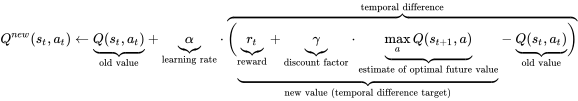
\includegraphics[scale=0.70]{images/qformula.png}
\caption{Update regel - Source: \cite{q-updaterule}}
\label{fig:qfunction}
\end{figure}
\noindent Er zijn nog een aantal belangrijke parameters aanwezig in de formule: 
\begin{itemize}
	\item Learning rate: Geeft aan in welke mate we de Q-waarde updaten, een grote learning rate zal dus meer impact hebben op de uiteindelijke Q-waarde dan een kleinere.
	\item Reward: Score die wordt berekend op basis van de state en de gekozen actie. Door deze actie uit te voeren, komen we in een nieuwe state en kunnen we aan de hand van een reward functie een score toekennen aan deze overgang. 
	\item Discount factor: Geeft aan hoe belangrijk toekomstige rewards zijn. Een hoge discount factor zal meer belang hechten aan rewards verder in de toekomst, een lage discount factor laat het algoritme enkel rewards in een korte tijdsperiode beschouwen.
	\item Estimate of optimal future value: In deze stap gaan we de Q-waarden overlopen over alle mogelijke acties in de volgende state, en halen we de hoogste Q-waarde eruit.
\end{itemize}
Bovendien is het in Q-learning belangrijk om te beschouwen hoe we de volgende actie $a$ kiezen, om dan overeenkomende $Q(s,a)$ aan te passen. We zouden elke keer de beste actie kunnen kiezen op basis van de Q-waarden, maar dit zal in begin niet werken, aangezien er dan nog helemaal niets geleerd is. Er moet genoeg exploratie zijn, zeker in het begin! Een oplossing hiervoor is om een $\epsilon$-greedy policy te volgen, waarbij we met kans $\epsilon$ een willekeurige actie kiezen, en met kans $1-\epsilon$ een actie kiezen gebaseerd op de huidige policy. Deze $\epsilon$ kan eventueel variëren met de tijd aan de hand van een $\epsilon$-decay factor.
\subsubsection{Implementatie}
De Q-waarden die doorheen het algoritme worden geüpdate, worden bijgehouden in een Q-table. In onze eerste implementatie houdt de state 2 velden bij die de rang van de laatst gelegde kaart en zijn hoeveelheid voorstellen. De state wordt gegeven als een tuple $(rang, aantal)$, en acties worden op dezelfde manier voorgesteld. Met deze 2 tuples indexeren we de Q-table.\\\\
We kunnen natuurlijk bediscussiëren of het niet beter zou zijn om een grotere state bij te houden, maar hier komen we later bij de resultaten op terug.\\\\
De initiële Q-waarden in de tabel zijn 0 voor alle acties behalve 'skip'. Met $skip$ wordt een beurt passen bedoeld. De waarden voor $skip$ in elke mogelijke state wordt op -1 gezet, wat betekent dat die al vanaf het begin wordt afgestrafd. Op deze manier proberen we ervoor te zorgen dat de agent in het begin zo veel mogelijk beslist om wel een kaart te leggen. \\\\
De Q-waarden updaten werkt als volgt. Wanneer het aan de agent is kiest hij een actie, die wordt opgeslaan samen met de huidige state. Daarna wordt de ronde verder gespeeld tot het terug aan hem is, waarbij hij dus in een nieuwe state terecht komt. Op basis van de vorige state, de actie en de nieuwe state wordt de reward berekend en de Q-table aangepast. De reward functie, optimale learning rate en discount factor bespreken we ook in de resultaten. \\\\
Voor de $\epsilon$ kiezen we als startwaarde 1 en na ieder actie zal de huidige $\epsilon$ vermenigvuldigd worden met een $epsilon\_decay$ parameter. Op deze manier is er in het begin van het trainen meer exploratie, maar zal $\epsilon$ afnemen en zullen we meer exploitatie hebben. Eenmaal $\epsilon = 0.05$ zal de $\epsilon$ niet meer verminderen, omdat we nog steeds wat exploratie willen hebben. In appendix \ref{appendix:epsilon} bespreken we de $\epsilon$-decay in meer detail.\\\\
In een poging om geheugen te besparen als we met grote states en acties werken, hebben we geprobeerd de states en acties in een bitvector vorm voor te stellen. Dit verminderde de performantie van het trainen en gaf geen significante verbeteringen in de prestatie van de agent. We hebben daarom dit idee gelaten voor wat het is.

\subsection{Deep Q-Network}
\subsubsection{Theorie}
In plaats van een tabel volledig op te slaan, benaderen we in het DQN-algoritme de tabel met een functie-approximator, wat hier een neuraal netwerk is.\\\\
Het updaten van dit neuraal netwerk werkt dan als volgt. Stel dat de agent zich bevindt in een toestand $s$, dan wordt er een actie $a$ gekozen op basis van een $\epsilon$-greedy policy (hier kan dat ook met $\epsilon$-decay). Door deze actie uit te voeren, komen we in een nieuwe state $s'$ terecht en wordt daarvoor een reward $r$ gegegeven. Bij Q-learning kunnne we hiermee de Q-table updaten, maar hier is het niet zo simpel. Merk wel op dat hier de discount factor en learning rate ook een belangrijke rol spelen, net zoals bij Q-learning.\\\\
De volgende stap is om deze originele state, de actie, de nieuwe state en de reward op te slaan in een replay memory. In dit replay memory krijgen we een verzameling van tuples van de vorm $(s,a,r,s')$. In elke stap worden samples uit het replay memory genomen en worden er voor deze samples $targets$ opgesteld. Deze targets worden op dezelfde manier berekend als de temporal difference targets bij Q-learning (zie Figuur \ref{fig:qfunction}). De targets zijn van de vorm `reward + estimate of optimal future value', de tweede term is niet meer nodig als we aan het einde van de episode zijn. In dit geval houden we enkel de reward over als target.\\\\
Daarna wordt het netwerk geüpdate aan de hand van een gradient descent stap, met een loss functie die de net berekende targets en de huidige Q-waarden van de samples gebruikt. Daarop kan ook nog een optimalisatie stap volgen. Er zijn verschillende loss en optimalisatie functies die gebruikt kunnen worden. Het trainen van het netwerk aan de hand van samples uit het replay memory wordt ook wel experience replay genoemd.

\subsubsection{Implementatie}
Er zijn al een aantal frameworks ter beschikking die ons een handje kunnen helpen. Wij hebben gekozen voor PyTorch, die de implementatie al een deel voor zich neemt. Belangrijke functies die we gebruiken voor het neuraal netwerk zijn de ADAM optimiser, de RELU activatie functie, en de MSE loss functie.\\\\
Als initiële state worden de kaarten in de hand en de laatst gelegde kaart(en) bijgehouden. De state bevat dan 15 velden, waarvan de eerste 13 velden aangeven hoeveel kaarten je van elke rang in je hand hebt. De laatste 2 stellen de laatste zet voor (met speciale waarden voor een skip en het begin van een ronde). Om deze velden te normaliseren voordat ze als input aan het neuraal netwerk worden gegeven, gebruiken we $aantal = (aantal - 2)/2$ om het aantal kaarten van een rang voor te stellen.\\\\
Na de input laag hebben we 2 hidden layers van elk 64 nodes. Daarop volgen 53 output nodes die elk een actie voorstellen. Er is dus een mapping van 0 tot 52 naar een zet die bestaat uit een aantal kaarten van een bepaalde rang. Deze zet kan ook een $skip$ zijn. Om de output te beperken, kan de agent maar hoogstens 4 kaarten leggen (ookal is het mogelijk om met jokers meer te leggen).\\\\
Net zoals bij de implementatie van Q-learning kiezen we hier voor een minimale $\epsilon$ van 0.05, startende bij 1. Belangrijke parameters zoals de discount factor en learning rate, en de reward functie bespreken we in detail bij de resultaten.

\section{Resultaten}
Om een gevoel te krijgen hoe goed een agent presteert gebruiken we een win/lose ratio. Dit zal enkel rekening houden met hoeveel een agent president is:
\begin{center}
$W/L = games\_president/total\_games\_played * 100$.
\end{center}
We vermenigvuldigen met 100 om het resultaat als percentage uit te drukken. Dit is een goede maat aangezien we hieruit ook kunnen afleiden dat als hij veel president is, hij waarschijnlijk ook vaak vice-president is, en minder scum of high-scum. Het is echter geen perfecte maat, omdat winnen niet altijd betekent dat de agent goed heeft gespeeld, zoals besproken in deel \ref{sec:env}.

\subsection{Heuristiek en random}
Het is belangrijk om te weten hoe de heuristieke speler het doet tegenover random spelers, en omgekeerd. Zo kunnen we goed vergelijken en hopelijk zelfs streven naar gelijkaardige of betere resultaten.
\begin{table}[H]
        \centering
        \resizebox{9cm}{!}{
        \begin{tabular}{|c|c|c|}
                \hline
                  vs                & 3 heuristieke spelers & 3 random spelers \\
                \hline
                 heuristieke speler & 25         & 65\\
                 random spelers     & 6         & 25\\
                \hline
        \end{tabular}
        }
        \caption{W/L in \% voor heuristieke agents}
\end{table}
\noindent In bovenstaande tabel zien we dat de heuristieke speler het al zeer goed doet, wat wel te verwachten was tegen random spelers. Een goed doel voor de reinforcement learning agents is dus minstens beter zijn dan de random speler of zelfs de heuristieke speler te evenaren, al dan niet te overtreffen.

\subsection{Q-learning}
\subsubsection{State met 2 velden}
Zoals beschreven in de implementatiedetails van Q-learning, werken we hier met een state die als $(rang, aantal)$ wordt voorgesteld. Dit is een redelijk beperkte state, waarvoor we een gepaste reward functie moeten vinden. Naast de reward functie kunnen de andere parameters ($\epsilon$, $\alpha$, $\gamma$) ook een invloed hebben.\\\\
We willen, net zoals bij de heuristieke speler, dat de agent een ronde zo goed mogelijk speelt en niet kijkt naar of hij president is geworden of niet. Dit vertaalt dan naar: de agent moet zo snel mogelijk al zijn kaarten uitspelen, of zo veel mogelijk kaarten spelen per ronde. Hiervoor zijn we tot volgende reward functie gekomen:
\begin{center}
$r = amount\_of\_cards\_played * 0.5 + amount\_of\_cards\_played\_in\_round * 0.2$
\end{center}
De reward functie bevat ook de term $amount\_of\_cards\_played\_in\_round$. Ookal zit die term niet in de state, wordt hij gebruikt om acties die vaak leiden tot meer kaarten gespeeld in een ronde extra te belonen.\\\\
Met learning rate $\alpha = 0.1$ en discount factor $\gamma = 0.75$ (deze optimale parameters komen uit het onderzoek in appendix \ref{appendix:parameters}), behaalt de Q-learning agent volgende resultaten. 
\begin{table}[H]
        \centering
        \resizebox{13cm}{!}{
        \begin{tabular}{|c|c|c|}
                \hline
                  vs           & 3 heuristieke spelers & 3 random spelers \\
                \hline
                 Q-learning agent getraind tegen random spelers & 15.1  & 53.2\\
                 Q-learning agent getraind tegen heuristieke spelers & 15.4 & 52.7\\
                \hline
        \end{tabular}
        }
        \caption{W/L in \% voor Q-table agent}
\end{table}
\noindent Dit zijn vrij goede resultaten, aangezien de random speler slechts een 6\% en 25\% haalt in deze situaties. Ook tegen de heuristieke speler zijn dit redelijk goede resultaten, aangezien de heuristieke speler een voordeel heeft: hij legt enkel jokers als dat nodig is. De Q-learning agent houdt hier geen rekening mee, wat een gedeeltelijke verklaring kan zijn voor het lagere resultaat.
\begin{figure}[H]
    \centering
    \subfloat[met gesorteerde Q-table]{{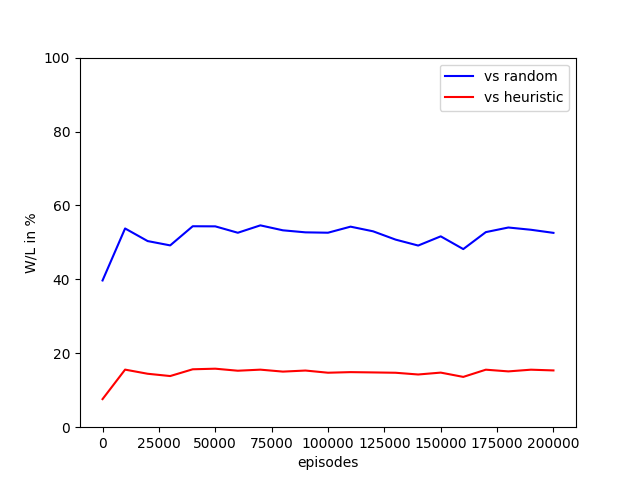
\includegraphics[width=7cm]{images/wins_in_time.png}} }
    \qquad
    \subfloat[alle versies van de Q-table tegen random spelers]{{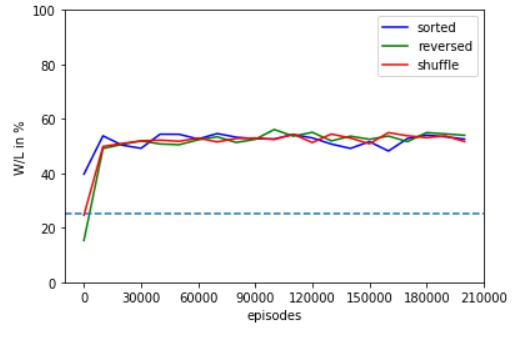
\includegraphics[width=7cm]{images/qtable-impl-random.png}} }
    \caption{Resultaten met $\gamma = 0.75$ en $\alpha = 0.1$ doorheen de tijd.}
    \label{fig:q_table_is_a_heuristic_player}
\end{figure}
\noindent De prestatie van de agent plotten voor meerdere episodes geeft een opmerkelijk resultaat. Namelijk dat de Q-learning agent de random agent sterk overtreft, zelfs zonder training! De oorzaak hiervan ligt bij de implementatie van de Q-learning agent. Als de agent een zet moet doen, worden alle mogelijke legale zetten gegenereerd voor de kaarten in zijn hand. Deze staan in volgorde van laagste kaarten naar hoogste kaarten. Als de Q-table nog maar net geïnitialiseerd is, staan alle Q-waarden op 0 en zal de agent de zet met de hoogste waarde nemen, namelijk de zet die als eerste is gegenereerd. Dit zal altijd de laagste kaart zijn. Dit op zich is al een kleine heuristiek die beter presteert dan de random keuze van de random agent. Met Q-learning kan de initialisatie van de Q-table en implementatie van acties kiezen dus de agent al een stapje vooruit helpen.\\\\
Om zeker te zijn dat de agent wel genoeg leert, hebben we ook het genereren van de zetten eens omgekeerd geïmplementeerd (zodat hij dus eerst de hoogst mogelijke kaarten legt) en het willekeurig kiezen uit zetten met de hoogste Q-waarde. Bij het laatste presteert hij precies even goed als de random spelers (streepjeslijn = 25\%). Dus hebben we hier, als alle waarden in de Q-table op 0 staan, een random agent via Q-learning geïmplementeerd. Na ongeveer 20 000 episodes convergeren deze implementaties, en blijven ze ongeveer stabiel rond de 50\%.

\subsubsection{Uitgebreide state}
Bij het testen van een Q-table met een grotere state waren de restulaten nooit zo goed als bij de kleinere Q-table. We merkten vaak op dat er delen van de Q-table helemaal niet geüpdate waren. Het probleem met een uitgebreide state, is dus dat er veel delen van de tabel niet of amper geëxploreerd kunnen worden, omdat de Q-table gewoonweg te groot wordt. Hierdoor zullen er veel Q-waarden niet aangepast zijn en nog op hun initiële waarde staan, waardoor de agent geen goede beslissing kan nemen. Bij presidenten is dit nog een groter probleem, aangezien het spel op zich meer zeldzame state-actie paren krijgt hoe meer de state uitbreidt, waardoor die zelfs nog minder bezocht worden.\\\\ 
Dit is dus een grote beperking van Q-learning. In appendix \ref{appendix:extended_state} is meer geschreven over de bevindingen van het experimenteren met een uitgebreide state, en geven we ook meer uitleg over die zeldzame state-actie paren bij presidenten.

\subsection{DQN}
Waar we nog niet in geslaagd zijn, is om de prestatie van de heuristieke speler te evenaren. Een mogelijke verklaring is de beperkte state, waarin we niet eens met de volledige hand kunnen rekening houden. Nu we werken met een deep Q-network, is het mogelijk om dit wel te doen.
\subsubsection{Klein DQN}
We hebben het over een $klein\ DQN$ als we werken met een state van 15 velden. De eerste 13 stellen de hand voor, de laatste 2 representeren de laatst gelegde kaart(en).  Dit is even veel informatie als de heuristieke speler heeft, wat we tot nu toe nog niet hebben kunnen bereiken op een functionele manier.\\\\
Als eerste testen we de reward functie die al goed heeft gepresteerd bij Q-learning. In deze context lijkt die niet zo succesvol te zijn, aangezien die ongeveer 24\% W/L geeft tegen 3 random spelers. Omdat we nu de volledige hand in de state bijhouden, kunnen we misschien een betere reward functie construeren op basis van de hand. De reward functie ziet er als volgt uit:\\\\
\indent als uitgespeeld: $reward = 10$\\
\indent als gepast: $reward = skip\_penalty$\\
\indent anders: $reward = relative\_hand\_score$\\\\
De $skip\_penalty$ geeft een hogere straf als er in het begin van de ronde gepast wordt, dan als er op het einde gepast wordt. De $relative\_hand\_score$ geeft een mate van verbetering van de hand aan. Het idee hier achter is dat je zoveel mogelijk je hoge kaarten probeert te behouden (hier is een joker de hoogste rang), en dat alle kaarten leggen van een rang beter is dan minder te leggen. \\\\
We hebben deze functie niet in 1 keer gevonden, maar hebben veel verschillende moeten uittesten. Daarbij is de relatieve hand score een reward die meer gebaseerd is op het korte termijn gedrag van de agent, het is dus interessant om te kijken hoe de discount factor $\gamma$ hier een rol in speelt.
\begin{figure}[H]
\centering
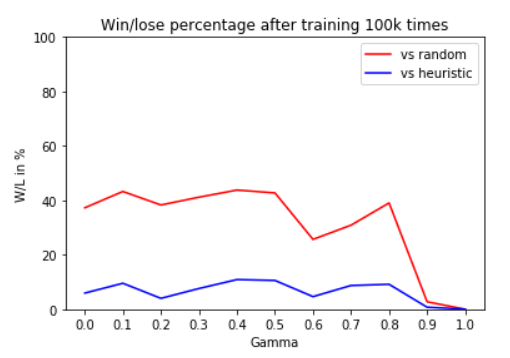
\includegraphics[scale=0.38]{images/gamma-iteratie-dqn.png}
\caption{Resultaten variëren van parameter $\gamma$}
\label{fig:gamma_iteratie_small_dqn}
\end{figure}
\noindent We zien dat hogere waarden van $\gamma$ de agent slechter doen presteren, op een punt met zelfs maar 0\% W/L. Door een hoge gamma zal het minder uitmaken wanneer de agent zijn hand verbeterd, en zal hij daarom vaker skippen, ookal krijgt hij daarvoor een straf.\\\\
\noindent Bovendien begint de winst te dalen voor $\gamma > 0.5$, maar na een tijdje stijgt die terug. Het is dus moeilijk om te besluiten of gamma best kleiner dan 0.9 of 0.5 moet zijn, of dat dit gewoon ligt aan schommelingen in het netwerk. Waarschijnlijk het laatste, aangezien de prestatie van het netwerk tijdens het trainen plotten (zie Figuur \ref{fig:kleine-dqn}) aantoont dat het vrij onstabiel is. Vermoedelijk heeft de learning rate $\alpha$ hier een invloed op.
\begin{figure}[H]
    \centering
    \subfloat[Resultaten variëren van parameter $\gamma$]{{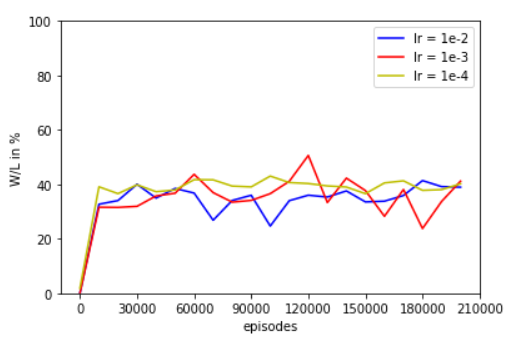
\includegraphics[width=7.5cm]{images/lr-iteration-random-small-dqn.png}} }
    \qquad
    \subfloat[tegen heuristieke spelers]{{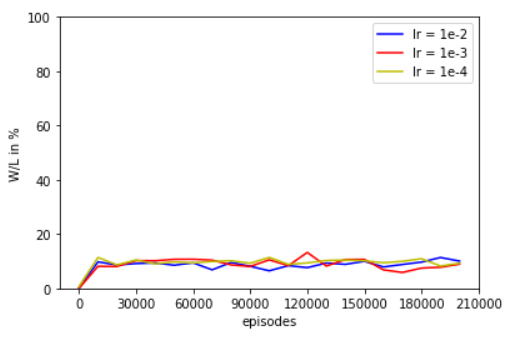
\includegraphics[width=7.5cm]{images/lr-iteration-heur-small-dqn.png}} }
    \caption{Resultaten met $\gamma = 0.5$ en $\alpha = \{0.01, 0.001, 0.0001\}$ doorheen de tijd.}
    \label{fig:kleine-dqn}
\end{figure}
\noindent Een lagere learning rate lijkt het netwerk inderdaad stabieler te maken, en geeft gemiddeld een betere prestatie. Met een hogere learning rate behalen we vaak slechtere resultaten en zijn er grote schommelingen. Een learning rate van 0.0001 is hier duidelijk beter. Op deze grafieken zien we ook dat na 20 000 episodes, het netwerk geconvergeerd lijkt te zijn en niet veel meer veranderd. \\\\
Nu de optimale parameters gekend zijn, kunnen de prestaties samengevat worden:
\begin{table}[H]
        \centering
         \resizebox{13cm}{!}{
        \begin{tabular}{|c|c|c|}
                \hline
                  vs           & 3 heuristieke spelers & 3 random spelers \\
                \hline
                 DQN agent getraind tegen random spelers & 9.8 & 39.5\\
                 DQN agent getraind tegen heuristieke spelers & 11.3 & 39.9\\
                \hline
        \end{tabular}
        }
        \caption{gemiddelde W/L in \% voor DQN agent met $\gamma=0.5$, $lr=0.0001$}
\end{table}
\noindent Merk op dat we met het construeren van een heel specifieke reward functie, maar een W/L percentage van ongeveer 40\% behalen tegenover de random spelers. Daarbij is het engineeren van een reward functie misschien niet de beste manier van aanpak. De agent volgt namelijk exact wat we aangeven in de reward functie, een kleine redeneringsfout kan de agent leiden tot heel vreemde acties.
\subsubsection{Groot DQN}
In het vorige deel hebben we een vrij gedetailleerde reward functie gemaakt, die elke stap een reward geeft. We willen echter de agent minder zelf sturen, en zelf de taktiek van het spel laten ontdekken. Daarvoor gebruiken we volgende, simpele reward functie:\\\\
\indent als president: $reward = 10$\\
\indent als vice-president: $reward = 5$\\
\indent als high-scum: $reward = -5$\\
\indent als scum: $reward = -10 - 3*amount\_cards\_in\_hand$\\
\indent anders: $reward = 0$\\

\noindent De agent krijgt dus enkel een reward op het einde van het spel. De state houdt vanaf nu ook alle gelegde kaarten bij in het spel. Er zijn 13 velden voor de eigen hand, 13 velden voor de gelegde kaarten in het spel, en 2 voor de laatst gelegde kaart(en). In totaal zijn dit 28 velden, waardoor we het $groot\ DQN$ noemen. Aangezien we nu enkel rewards geven voor de finale actie van een spel, vermoeden we dat een hogere gamma betere resultaten zal geven.
\begin{figure}[H]
    \centering
    \subfloat[na 20 000 episodes training]{{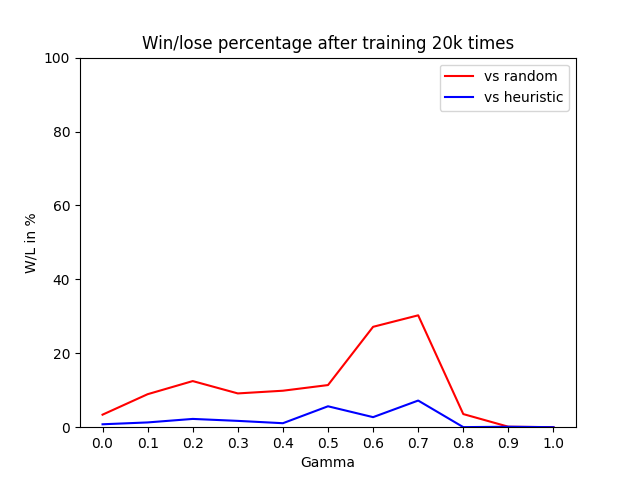
\includegraphics[width=6.9cm]{images/gamma_bigdqn_20k.png}} }
    \qquad
    \subfloat[na 100 000 episodes training]{{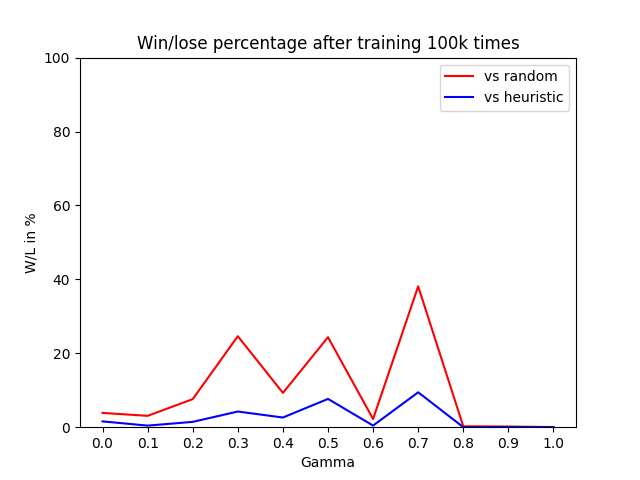
\includegraphics[width=6.9cm]{images/gamma_bigdqn_100k.png}} }
    \caption{Resultaten variëren van $\gamma$.}
\end{figure}
\noindent Bij het simuleren van het netwerk met verschillende waarden van $\gamma$, zien we dat voor lage $\gamma$ inderdaad lage resultaten worden behaald, maar de $\gamma$ mag ook niet te hoog zijn. Er zijn ook schommelingen te zien in de prestatie, waardoor het niet erg duidelijk is welke $\gamma$ exact het best zou presteren. Daarom moet opnieuw de invloed van de learning rate parameter onderzocht worden. 
\begin{figure}[H]
    \centering
    \subfloat[Variëren van learning rate]{{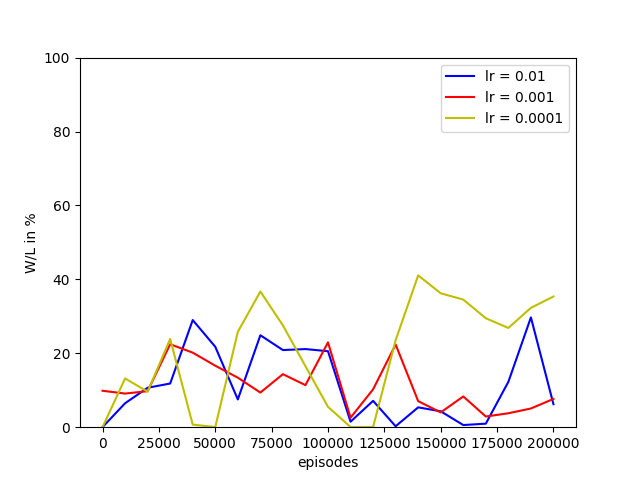
\includegraphics[width=6.9cm]{images/lr-iteration-random-big-dqn.png}} }
    \qquad
    \subfloat[Langer trainen met $lr = 0.0001$]{{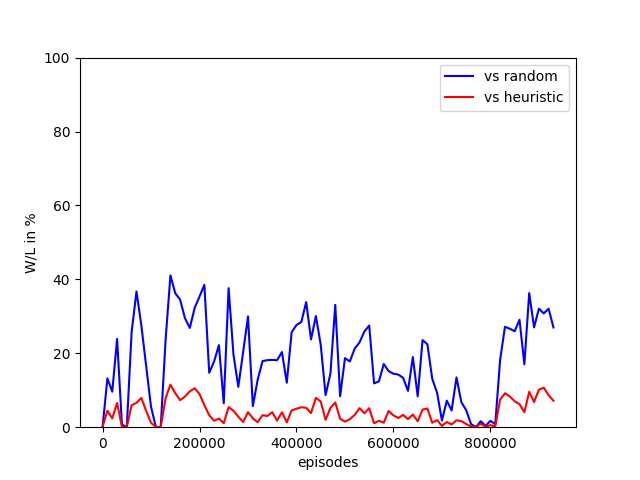
\includegraphics[width=6.9cm]{images/big_dqn_extended_training.png}} }
    \caption{Resultaten met $\gamma = 0.7$ doorheen de tijd.}
    \label{fig:results_bigdqn_in_time}
\end{figure}
\noindent Net als bij het klein DQN zien we opnieuw grote bewegingen in de prestatie, maar er is geen learning rate die een betere stabiliteit biedt. De oorzaak van deze grote schommelingen ligt ook niet bij het feit dat er nog niet genoeg is getraind (zie Figuur \ref{fig:results_bigdqn_in_time}(b)), met langere training is het netwerk nog steeds onstabiel: soms krijgen we een 5\% W/L en dan iets later een 42\% W/L. Wat nog opviel, was dat het trainen van het groot DQN al wat langer duurde dan het trainen van het klein DQN, wat wel te verwachten was.\\\\
Om zeker te zijn dat de onstabiliteit niet aan de random tegenstanders ligt, hebben we de agent ook laten trainen tegen 3 heuristieke spelers. Dit gaf zelfs nog mindere prestaties, er werd niet eens meer boven de 15\% W/L gehaald. Een verklaring hiervoor kan zijn dat de speler te weinig wint tegen de heuristiek, en vaak enkel negatieve rewards haalt, waardoor de agent niet echt leert wat hij wél moet doen.\\\\
Er zijn dus nog duidelijk problemen met de DQN aanpak, maar dit kan aan heel veel liggen. Het zou kunnen dat we de state beter hadden moeten voorstellen door bv. meer of minder velden te gebruiken. Ook de reward functie kan een grote invloed gespeeld hebben, het zou kunnen dat iets kleins zoals een negatieve reward geven bij high-scum het netwerk fout stuurt. Nog een mogelijk probleem kan overfitting zijn, waardoor de agent op heel specifieke situaties heeft leren spelen, en bij de rest volledig de mist in gaat. Werken met een neuraal netwerk is dus veel complexer en onvoorspelbaarder dan werken met een simpele Q-table, maar kan als alles zo optimaal mogelijk ingesteld is waarschijnlijk betere prestaties neerzetten.

\section{Conclusie}
Alhoewel geen enkel reinforcement learning algoritme de heuristieke speler heeft kunnen overtreffen, zijn de resultaten zeker niet slecht. Wat ons vooral heeft verbaasd, is dat het simpelere algoritme, Q-learning, het hier beter heeft gedaan. We hadden niet verwacht dat een simpele state met een simpele reward het zo goed zou kunnen doen. We zitten hier wel met een beperking, namelijk de Q-table die niet te groot mag worden.\\\\
Daarom zien we dus meer potentieel in de DQN agents, waarbij we een grotere state kunnen bijhouden en dus veel meer vrijheid hebben. Hierdoor kan er ook creatiever omgegaan worden met de reward functies, wat zeker een voordeel is. Alhoewel het vinden van een reward functie vrij simpel is, is het vinden van een echt goede reward functie niet zo simpel. Wat dit zo moeilijk maakt, is het feit dat het heel sterk beïvloedt hoe een agent presteert: een kleine redeneringsfout kan al snel een negatieve invloed hebben. Buiten de reward functie, valt er in het algemeen nog veel meer te experimenteren en uit te proberen bij het DQN-algoritme. Dit zou misschien op een punt betere prestaties kunnen leveren dan Q-learning met een Q-table. 
\newpage
\begin{thebibliography}{9}
\bibitem{simple-qlearning} 
Andrew Thomas. "Reinforcement learning tutorial using Python and Keras"
\\\texttt{https://adventuresinmachinelearning.com/reinforcement-learning-tutorial-python-keras/}

\bibitem{nn-paper} 
Henry Charlesworth. "Application of Self-Play Reinforcement Learning to a Four-Player Game of Imperfect Information" (2018) 
\\\texttt{https://arxiv.org/pdf/1808.10442.pdf}

\bibitem{mct-1} 
Sammie Katt and Frans A. Oliehoek and Christopher Amato. "Learning in POMDPs with Monte Carlo Tree Search" 
\\\texttt{http://proceedings.mlr.press/v70/katt17a/katt17a.pdf}

\bibitem{mct-2} 
Maxiem Wagenaar. "Learning to play the Game of Hearts using reinforcement Learning and a multi-layer perceptron"
\\\texttt{https://fse.studenttheses.ub.rug.nl/15440/1/Bachelor\_Thesis\_-\_Maxiem\_Wagen\_1.pdf}

\bibitem{mct-3} 
Ömer Baykal and Ferda Nur Alpsaslan. "Reinforcement Learning in Card Game Environments Using Monte Carlo Methods and Artificial Neural Networks" (2019)
\\\texttt{https://www.researchgate.net/publication/337508729\_Reinforcement\_Learning\_in\_Card\_Game\_}
\\\texttt{Environments\_Using\_Monte\_Carlo\_Methods\_and\_Artificial\_Neural\_Networks}

\bibitem{bellman-equations} 
Bellman Equations
\\\texttt{https://en.wikipedia.org/wiki/Bellman\_equation}

\bibitem{q-updaterule} 
Q-learning
\\\texttt{https://en.wikipedia.org/wiki/Q-learning}
\end{thebibliography}

\newpage


\appendix
\section{\\Learning rate en discount factor voor state met 2 velden}
% the \\ insures the section title is centered below the phrase: AppendixA
\label{appendix:parameters}
Voor de juiste learning rate $\alpha$ en discount factor $\gamma$ kunnen we simulaties laten lopen om zo de optimale parameters te vinden. Hieronder zien we de W/L voor alle mogelijke parameters voor $\alpha$ en $\gamma$ met stappen van $0.1$.
\begin{figure}[h]
\centering
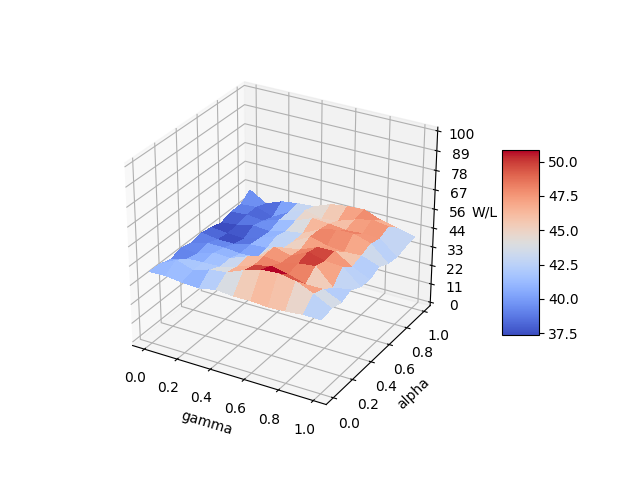
\includegraphics[scale=0.50]{images/qtable_parameter_random.png}
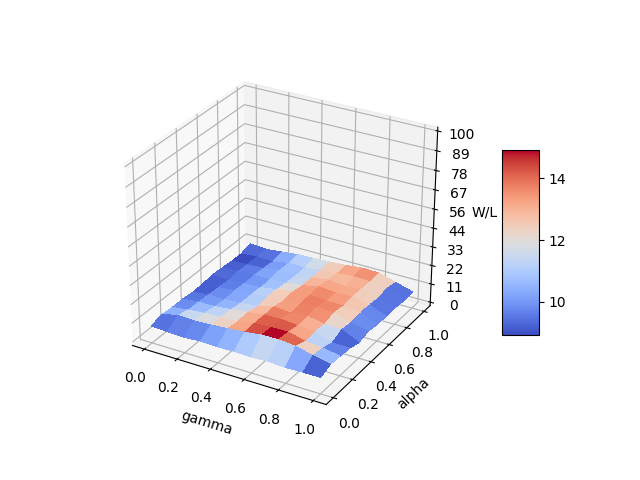
\includegraphics[scale=0.50]{images/qtable_parameter_heuristic.png}
\caption{Resultaten variëren met parameters $\gamma$ en $\alpha$ na 50000 episodes, links tegen random, rechts tegen heuristieke spelers}
\end{figure}
We zien nu dat er voor $\gamma \in [0.5, 0.8] $ en $\alpha \in [0.1, 0.3] $ meer winst wordt behaald. Bovenstaande figuren zijn bekomen met training van 50000 keer. We zullen nu dubbel zo veel trainen voor deze intervallen om zo de optimale $\gamma$ en $\alpha$ te vinden\\\\
\begin{figure}[h]
\centering
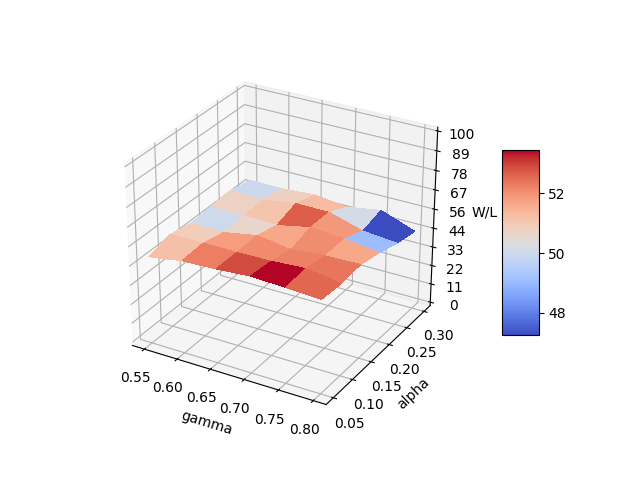
\includegraphics[scale=0.50]{images/qtable_parameter_random_zoomed.png}
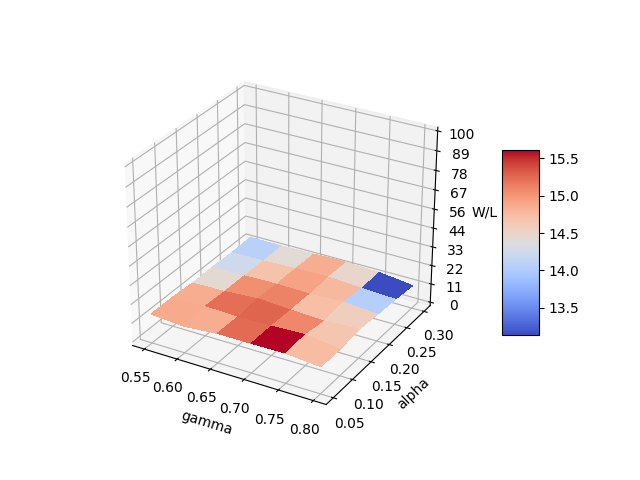
\includegraphics[scale=0.50]{images/qtable_parameter_heuristic_zoomed.png}
\caption{Resultaten variëren met parameters $\gamma$ en $\alpha$ na 100000 episodes, links tegen random, rechts tegen heuristieke spelers}
\end{figure}\\
Uit bovenstaande afbeeldingen kunnen we besluiten dat de optimale parameters, voor de gebruikte rewardfunctie, $\alpha = 0.1$ en $\gamma = 0.75$ zijn.

\section{\\Epsilon-decay}
\label{appendix:epsilon}
Aangezien we met $\epsilon$ decay werken, illustreren we hieronder dat het belangrijk is om je $epsilon\_decay$ factor dicht genoeg bij 1 te nemen. Anders zal $\epsilon$ al snel zijn minimum hebben bereikt en zal er misschien niet genoeg exploratie geweest zijn.\\
\begin{figure}[h]
\centering
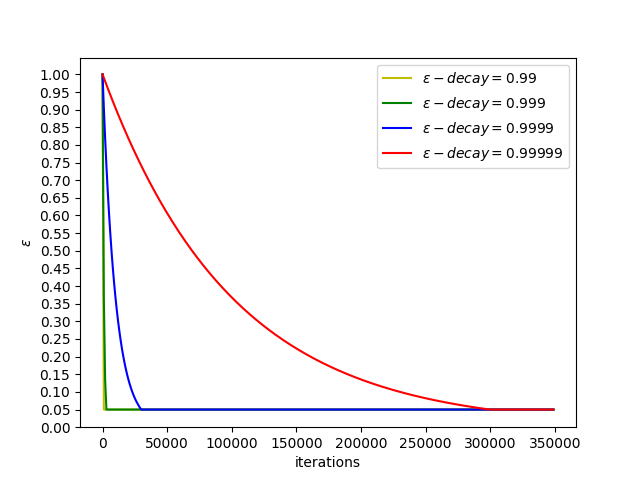
\includegraphics[scale=0.65]{images/epsilon_decay.png}
\caption{Illustratie van epsilondecay met een minimum $\epsilon$ van 0.05}
\end{figure}\\
Voor ons model kozen wij voor een $epsilon\_decay$ factor van 0.9999. Als we 100 000 episodes trainen, bereiken we de minimale epsilon dan na ongeveer 30 000 episodes. Dat betekent dat er na 30\% van de episodes voornamelijk exploitatie is. Het blijkt dat ons model al na 30 000 episodes geconvergeerd is. Daarom bekijken we of een kleinere $epsilon\_decay$ factor niet betere resultaten oplevert.\\\\
In onderstaande tabel staan de resultaten van simulaties gedaan voor de $epsilon\_decay$ factoren uit bovenstaande grafiek, voor een model met $\alpha = 0.1$ en $\gamma = 0.75$ (zie appendix \ref{appendix:parameters})
\begin{table}[H]
        \centering
        \begin{tabular}{|c|c|c|c|c|}
                \hline
                                & 0.99&0.999&0.9999&0.99999\\
                                \hline
                3 random speler  &52.83&50.65&51.1&52.41\\
                3 heuristieke spelers      &14.77&14.87&14.49&15.12\\
                \hline
        \end{tabular}
        \caption{W/L voor Q-table agent in \% voor verschillende epsilon-decay factoren na 100 000 episodes}
\end{table}
\noindent We zien dat zelfs voor een $epsilon\_decay$ factor van 0.99 de agent even goed presteert als onze initiële agent die met 0.9999 is getraind. Ook voor $epsilon\_decay = 0.99999$, waarbij er nog veel exploratie is na 100 000 episodes, is dit het geval. We kunnen dus besluiten dat de $\epsilon$ en $epsilon\_decay$ parameters een beperkte invloed hebben op de prestatie van de agent.\\\\

\section{\\Q-Table met uitgebreide state}
\label{appendix:extended_state}
Idealiter bevat de state van de agent ook de kaarten in je hand. Dit gaat alweer iets meer naar de richting de heuristieke speler, die ook op basis van zijn hand een beslissing maakt. Na wat zorgvuldig rekenwerk zou dit neerkomen op 2872 mogelijke starthanden, nog zonder alle mogelijke states na het leggen van 1,2,... kaarten. Dit zijn heel veel states! Er moet dus veralgemeend worden, zoals het bijhouden van het aantal kaarten in je hand, en niet de kaarten exact.\\\\
We kunnen de state als volgt voorstellen: $(rang, aantal, aantal\_kaarten\_in\_hand)$. Met de reward functie die hierboven zo goede resultaten gaf, krijgen we nu nog maar rond de 30\% W/L tegen 3 random spelers. Dit is dus niet veel beter meer dan een random agent.\\\\
We kunnen de state nog meer proberen veralgemenen. Als we werken met een state\\\\
\indent $(rang, aantal, aantal\_kaarten\_in\_hand)$ met
\begin{center}
$aantal\_kaarten\_in\_hand = aantal$ $if$ $ aantal <= 4$ $else$ $5$
\end{center}
En we initialiseren de state-actie paren op 10 voor de acties op een state die de zorgen dat de speler uitspeelt. Gebruikmakend van dezelfde reward functie als de kleine Q-table, behalen we een W/L van 40\% tegen random spelers. Dit is al een verbetering, maar is duidelijk nog niet beter dan de kleine Q-table. Het valt op dat een grotere Q-table slechtere resultaten geeft. Er is dus een punt dat de Q-table te groot wordt om hem nog volledig of genoeg te kunnen exploreren.\\\\
Bij presidenten komt er dan nog een extra probleem, namelijk dat er heel wat zeldzame states en bijhorende acties zijn, vooral als je de state uitbreidt. Het zal bijvoorbeeld niet erg veel voorkomen dat je 4 koningen kan leggen, waardoor de Q-waarde van deze actie niet veel aangepast gaat worden bij het trainen, en nog minder als deze actie over veel states kan gedaan worden (dus in het geval van een grote Q-table).\\\\
Als we dan positieve rewards geven, en we beginnen met alle state-actie waarden op 0, dan worden de waarden van de vaak voorkomende state-actie paren groter dan de waarden van zeldzame paren. Echter zijn vaak de zeldzame zetten zeer goed, maar zullen ze niet genomen worden omdat ze een lagere Q-waarde hebben. \\\\
Neem als voorbeeld dat de state bestaat uit $(rang, aantal, aantal\_kaarten\_in\_hand)$ en (3,2,4) is. Onze agent heeft 3 Q'en en een A in zijn hand. De beste zet is de 3 Q'en leggen, waarmee de ronde waarschijnlijk gewonnen zou worden, en dan de A leggen waarmee hij het spel wint. Maar, de actie 3Q zal voor een hand van 4 kaarten hoogstwaarschijnlijk nog niet of nog maar heel weinig zijn voorgekomen waardoor dit een lagere Q-waarde zal hebben dan bijvoorbeeld 1Q leggen in het geval dat je nog maar 4 kaarten hebt. Daarom zal de agent niet de optimale actie kiezen.\\\\
We kunnen ook negatieve rewards geven, en alles initialiseren op 0. Stel de agent heeft alle 4 de jokers. Dit komt zelden voor, waardoor de Q-waarde nog een redelijk "hoge" waarde dicht bij 0 zal hebben. Dit betekent dat de agent het leggen van de 4 jokers in 1 zet als een goede actie ziet. Dit is echter niet het geval want dan is hij zijn 4 jokers kwijt. Bij een te grote Q-table kan het dus zijn dat deze actie bij veel states nog niet is voorgekomen.
\end{document}
